\documentclass{beamer}

\usecolortheme[light]{solarized}
\setbeamertemplate{navigation symbols}{}%remove navigation symbols

\usepackage{tikz}
\usepackage{hyperref}
\usepackage{pgfgantt}
\usetikzlibrary{calc, shapes}

\title{Presentations}
\date{}
\author{}

\begin{document}

\frame{\titlepage}

\frame{
    \Huge
\begin{itemize}
    \item Ground council pitch
    \item Team presentations
\end{itemize}

}


\frame{
    \Large{
        \begin{center}
            How do you prepare for a pitch?
        \end{center}
    }
}


\frame{
    \begin{center}
        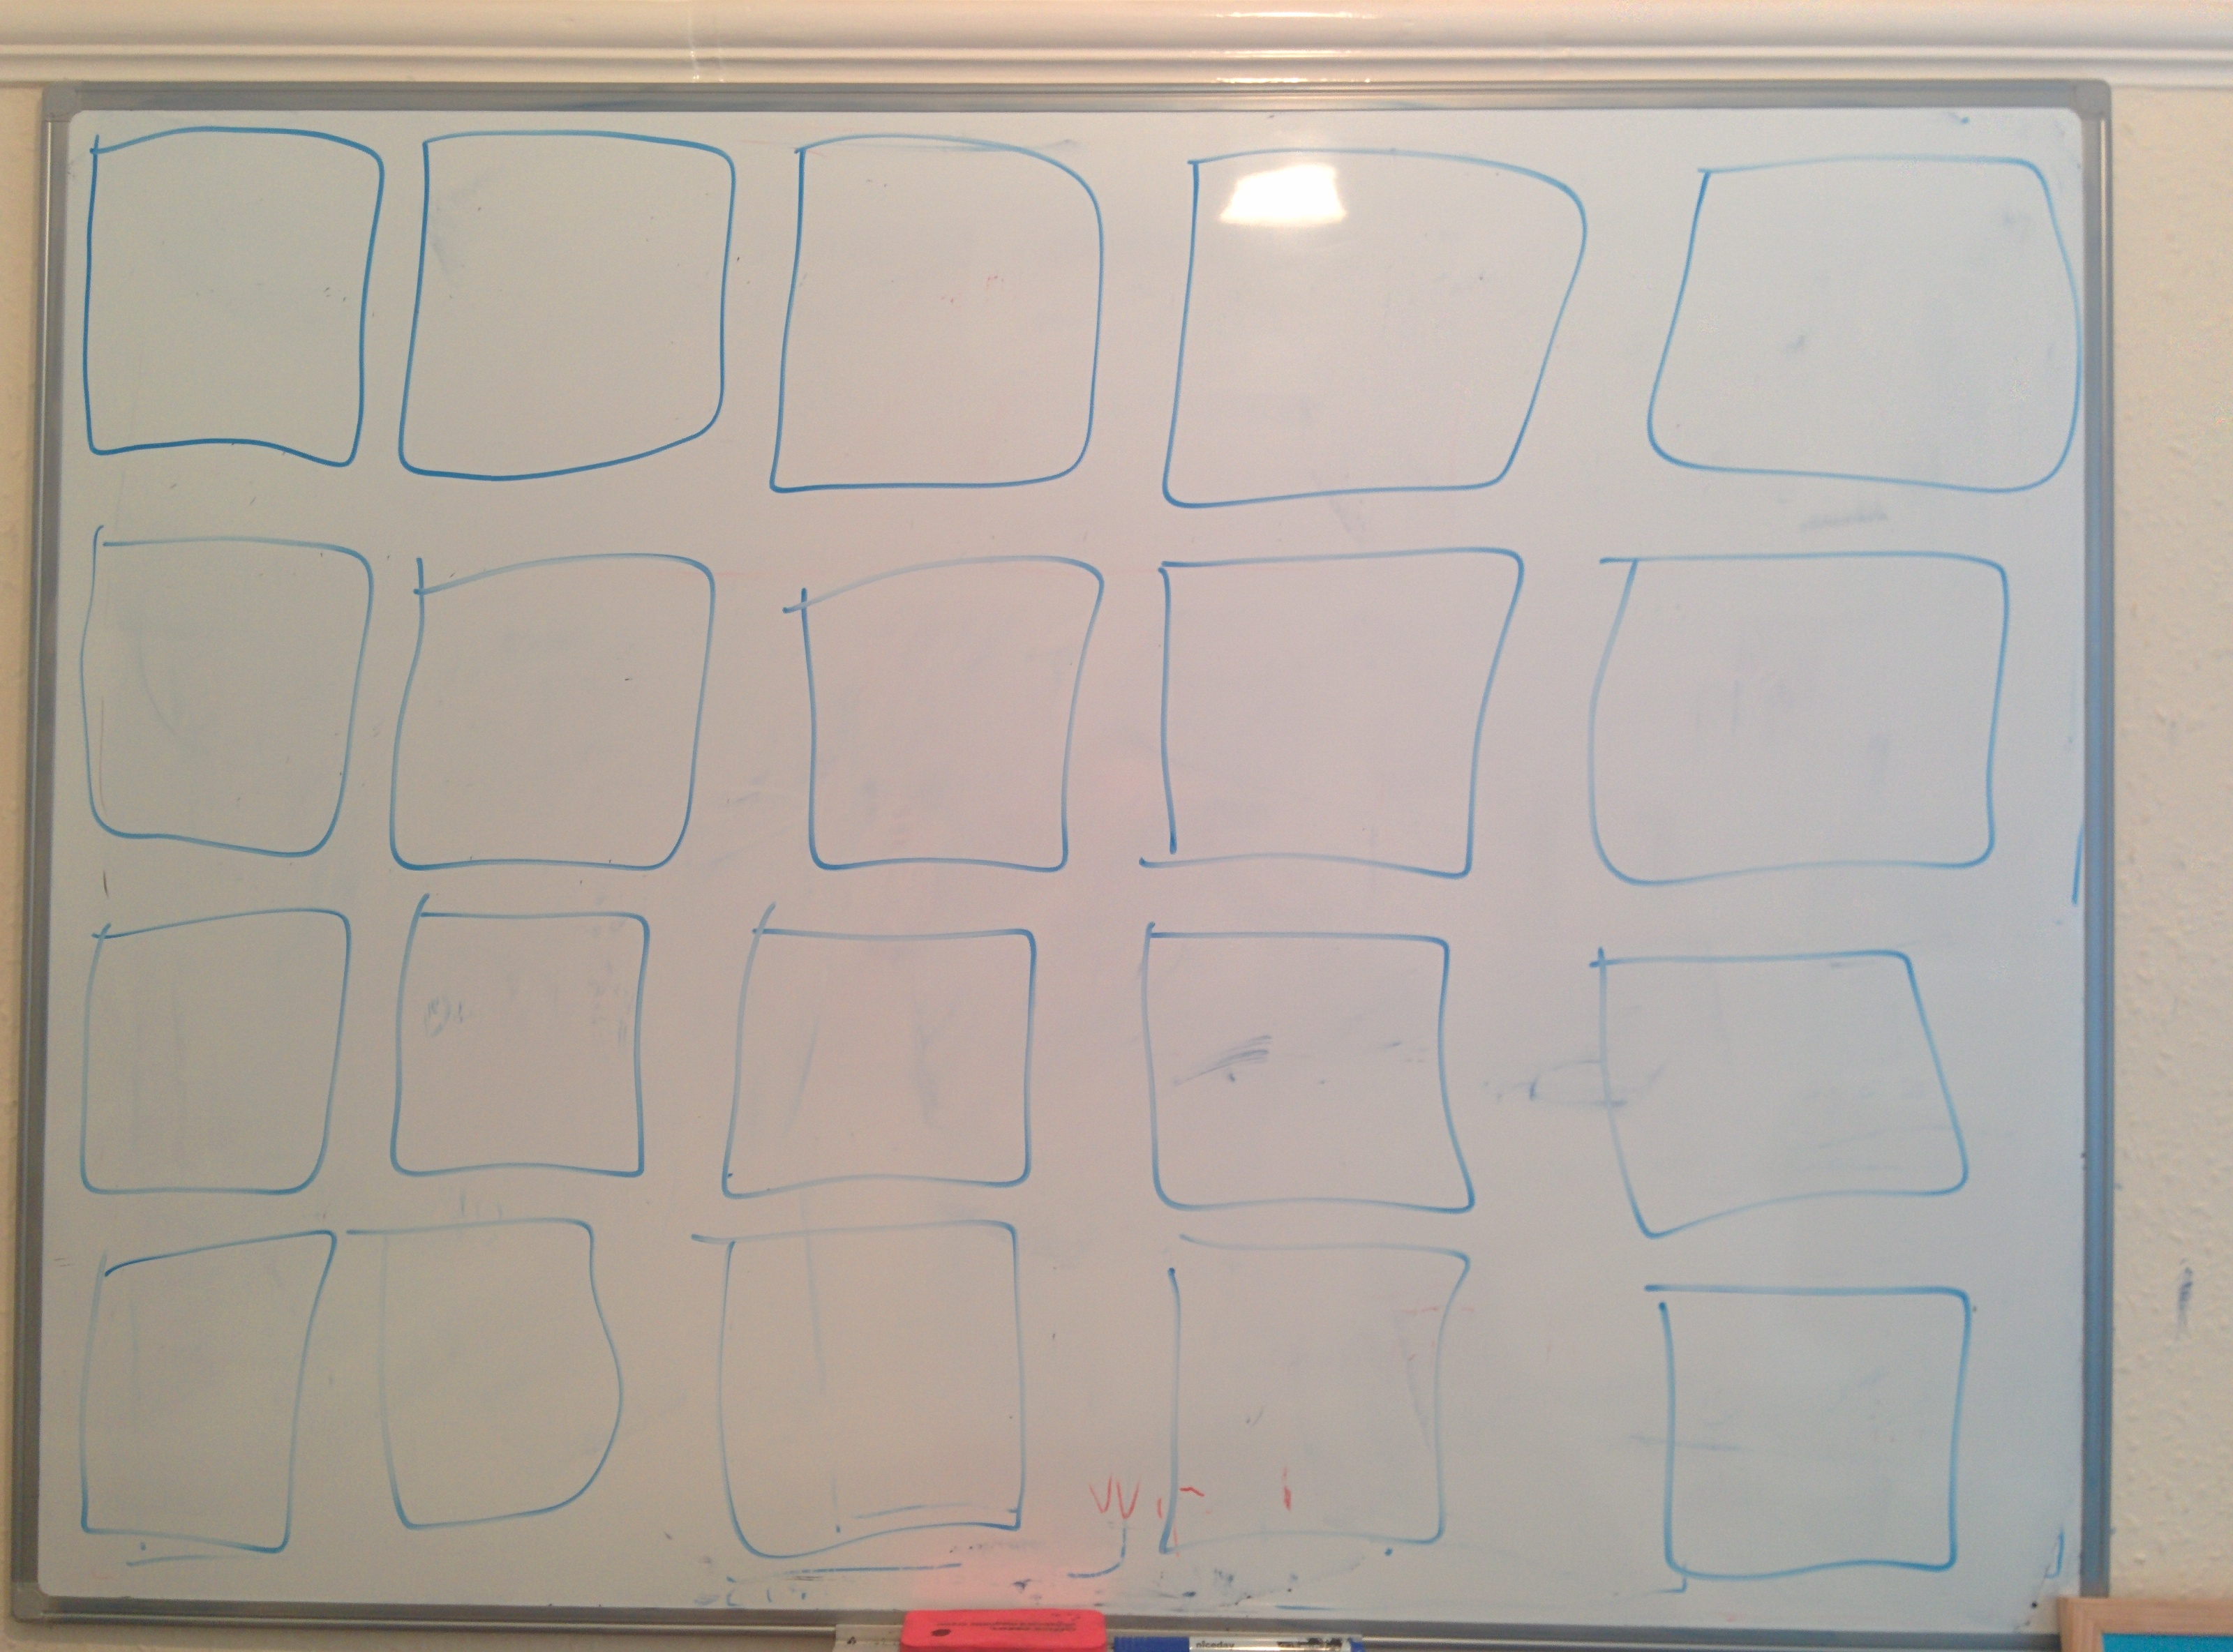
\includegraphics[width=.8\textwidth]{storyboard.jpg}
    \end{center}
}


\frame{
    \begin{center}
        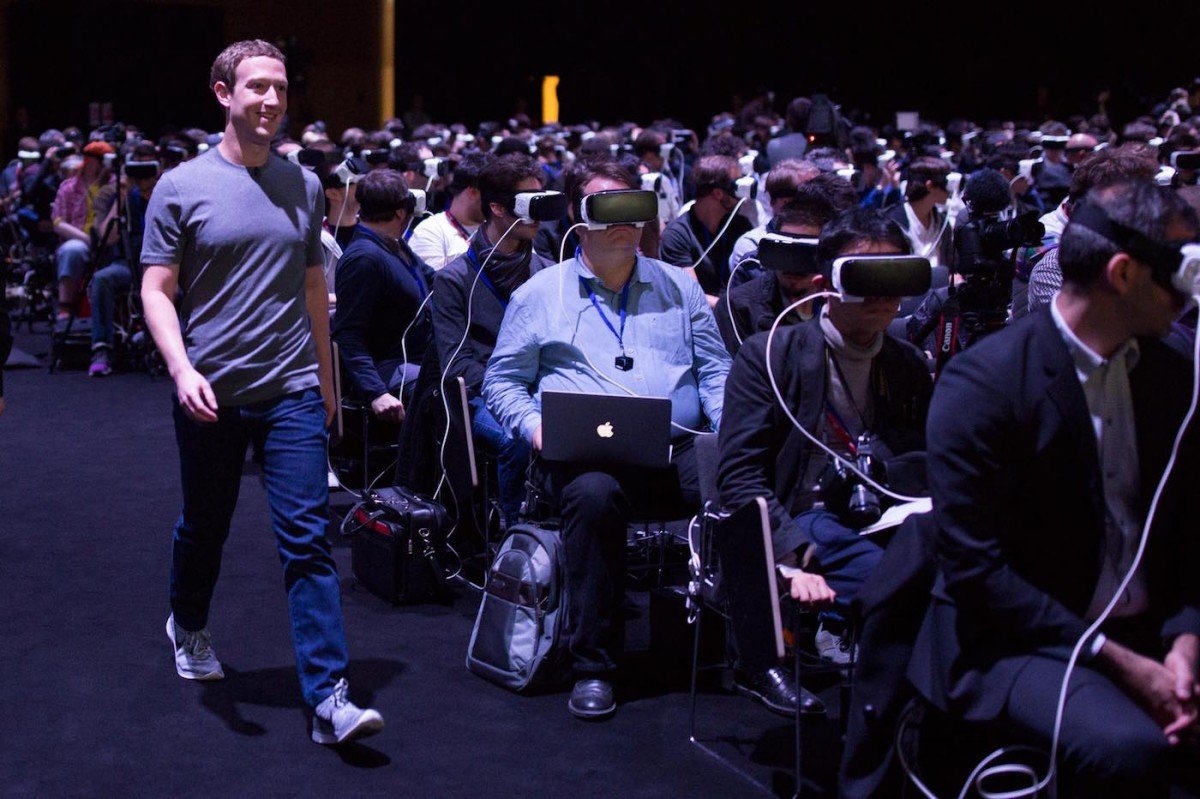
\includegraphics[width=.8\textwidth]{audience.jpg}
    \end{center}
}

\frame{
    \frametitle{Ways to fail}
    \begin{itemize}
        \item Voice and tone;
        \item Lack of passion;
        \item Hiding behind notes;
        \item Hands in pockets;
        \item Not looking interested when others are talking.
    \end{itemize}
}

\frame{
    \begin{itemize}
        \item Do
        \item not
        \item use
        \item bullet
        \item point
        \item after
        \item bullet
        \item point
        \item after
        \item bullet
        \item point
        \item after
        \item bullet
        \item point.
    \end{itemize}
}

\frame{
    Don't put so much text on the slide that the font size is so small that
    people can't read your information. Also, if you put a lot of text on the
    slide, people will be reading the slide instead of listening to the speaker
    just as you are now. See what I mean? What did I say just now? Were you
    reading or listening to me? You think people are listening to you but they
    are trying to read the information just before you flip to the next slide
    and they then they don't get either what is on the slide or what you have
    said. If you do this with most of your slides, people will stop trying to
    listen to read or hear what you are saying and will either daydream or
    leave. So limit the number of words. These slides are visual aids: they are
    meant to support what you are saying. Perhaps I've just told you where I am
    from and you missed it because you were reading this. A slide with an image
    of the country would have been far better as a way to complement what I was
    saying.
}

\frame{
    \begin{center}
        
\includegraphics[width=.8\textwidth]{fiji.jpg}
    \end{center}
}

\frame{
    \begin{center}
        \url{https://www.youtube.com/watch?v=1jkGw5VIC-c}
    \end{center}
}

\frame{
    \begin{center}
        \url{https://www.youtube.com/watch?time_continue=1&v=vKFJ_AI3PWA}
    \end{center}
}

\frame{
    \begin{center}
        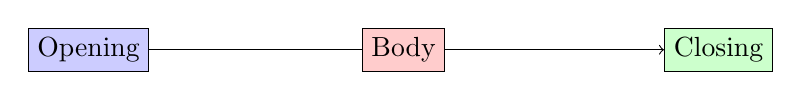
\begin{tikzpicture}
            \node (A) at (0,0) [fill=blue!20, draw] {Opening};
            \node (B) at (4,0) [fill=red!20, draw] {Body};
            \node (C) at (8,0) [fill=green!20, draw] {Closing};

            \draw [->] (A) -- (B) -- (C);
        \end{tikzpicture}
    \end{center}
}

\frame{
    \frametitle{Grand Council (\textbf{1 minute!})}

    \begin{enumerate}
        \item Who are you?
        \item Why do you need to solve the problem you are trying to solve?
        \item What does your company do to solve the problem? What's your value
            proposition? What makes you different (USP)?
    \end{enumerate}
}

\frame{
    \begin{center}
        \url{https://www.youtube.com/watch?v=Tq0tan49rmc}
    \end{center}
}

\frame{
    \begin{center}
        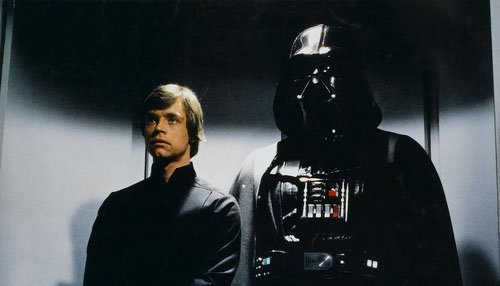
\includegraphics[width=.8\textwidth]{elevator.jpg}
    \pause

    Prep: 2 mins; Pitch: 1 min.
    \end{center}
}

\frame{
    \begin{center}
        \url{https://www.youtube.com/watch?v=v2w_a1wAo_M}
    \end{center}
}

\frame{
    \begin{center}
        \Huge Preparation
    \end{center}
}


\frame{
    \begin{center}
        \Huge Color and clarity
    \end{center}
}

\frame{
    \frametitle{Creating visual \textbf{aids}}

    \begin{itemize}
        \item Powerpoint;
        \item Prezzi;
        \item Beamer;
        \item Reveal (\url{http://lab.hakim.se/reveal-js/}).
        \item Inkscape.
    \end{itemize}

    \pause
    \begin{center}
        (Some examples (with source code): \url{http://vknight.org/Talks/})
    \end{center}
}
\end{document}
